% Copyright page
\makeatletter
\uppertitleback{\@titlehead}
\lowertitleback{
    \textbf{Pas de copyright} \\
    \ccby\ Ce mémoire est mis à disposition selon les termes de la
    \href{https://creativecommons.org/licenses/by/3.0/fr/}{Licence \en{Creative Commons Attribution}}.

    \medskip

    \textbf{Colophon} \\
    Ce document a été composé avec l'aide de
    \href{https://sourceforge.net/projects/koma-script/}{\KOMAScript} et
    \href{https://www.latex-project.org/}{\LaTeX} en utilisant la classe
    \href{https://github.com/fmarotta/kaobook/}{kaobook}.

    \medskip

    \textbf{Éditeur} \\
    Première publication le \todo[inline]{TODO} par l'Université de Strasbourg
}
\makeatother

% TODO: should it be included in the PDF?
% 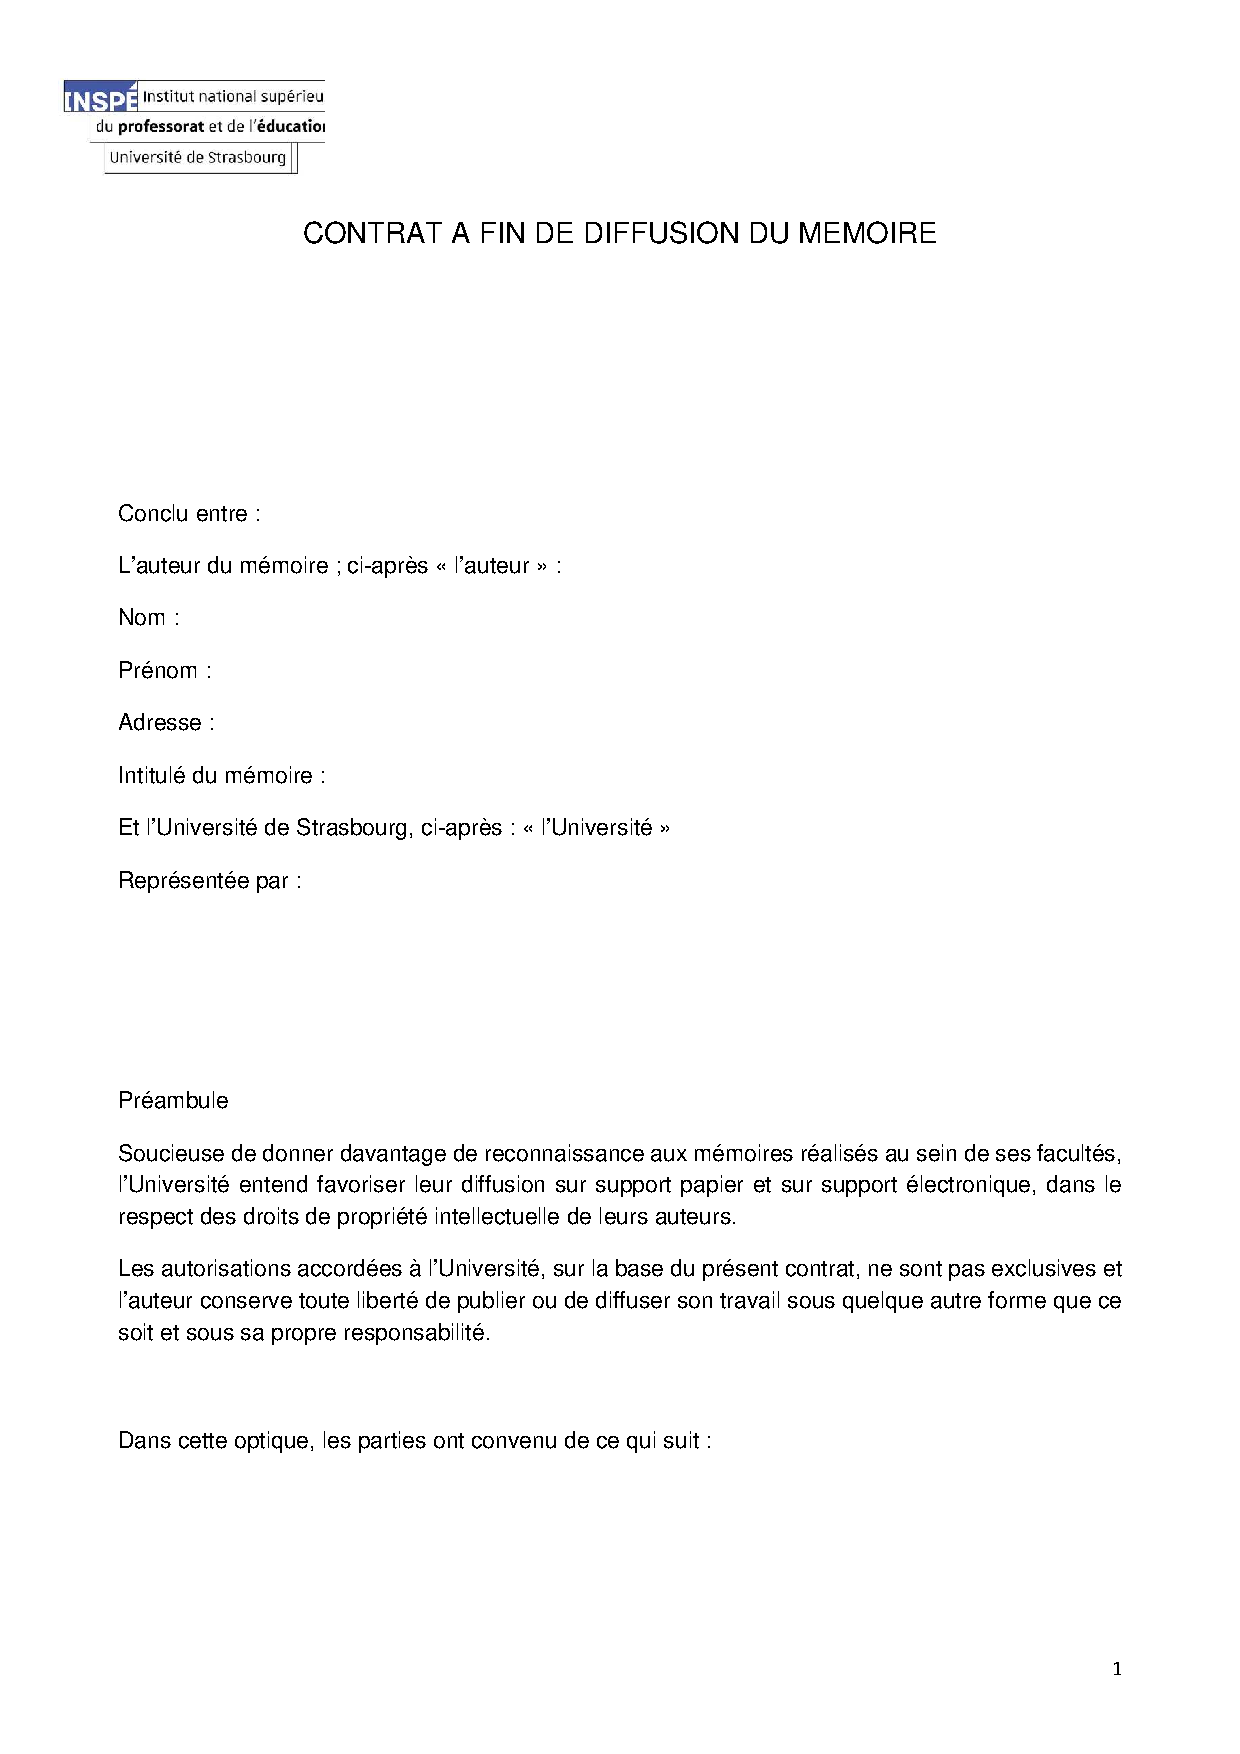
\includepdf[pages=-]{contrat_diffusion.pdf}

% Note that \maketitle outputs the pages before here
\maketitle

% Table of contents, figures and tables
\begingroup % Local scope for the following commands
    % Replace the automatic page break between those lists by a simple vertical split
    \newcommand{\biggerskip}{\vspace{4\bigskipamount}}
    \let\cleardoublepage\biggerskip
    \let\clearpage\biggerskip

    \tableofcontents
    \listoffigures
    \listoftables
\endgroup
